% CDF Dice

\documentclass[tikz = true, border = 2pt]{standalone}
\usepackage{tikz}
\usepackage{xfrac}
\usepackage{fontspec}
\setmainfont{Equity Text A}

\definecolor{firebrick}{RGB}{205,38,38}
\definecolor{royalblue}{RGB}{67,110,238}

\tikzset{
	dot hidden/.style={},
	line hidden/.style={},
	dot colour/.style={dot hidden/.append style={color=#1}},
	dot colour/.default=black,
	line colour/.style={line hidden/.append style={color=#1}},
	line colour/.default=black
}

\NewDocumentCommand{\drawdie}{O{}m}{
	\begin{tikzpicture}[x=1em,y=1em,radius=0.1,#1]
	\draw[rounded corners=2,line hidden] (0,0) rectangle (1,1);
	\ifodd#2
	\fill[dot hidden] (0.5,0.5) circle;
	\fi
	\ifnum#2>1
	\fill[dot hidden] (0.25,0.25) circle;
	\fill[dot hidden] (0.75,0.75) circle;
	\ifnum#2>3
	\fill[dot hidden] (0.25,0.75) circle;
	\fill[dot hidden] (0.75,0.25) circle;
	\ifnum#2>5
	\fill[dot hidden] (0.75,0.5) circle;
	\fill[dot hidden] (0.25,0.5) circle;
	\ifnum#2>7
	\fill[dot hidden] (0.5,0.75) circle;
	\fill[dot hidden] (0.5,0.25) circle;
	\fi
	\fi
	\fi
	\fi
	\end{tikzpicture}
}

\begin{document}

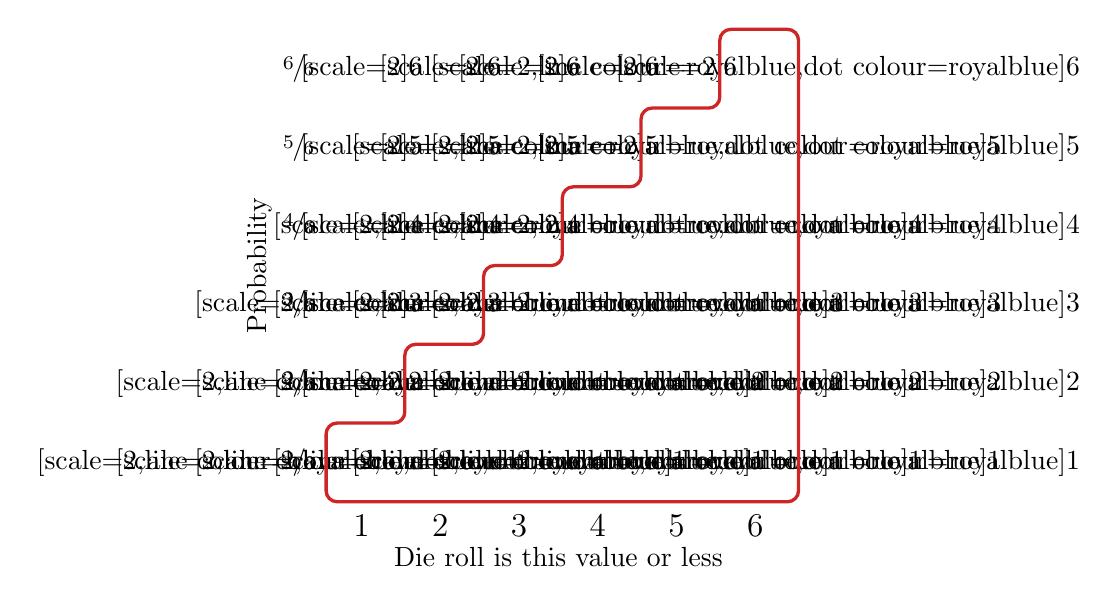
\begin{tikzpicture}
\foreach \i in {1,...,6} {
	\node at (0.2,\i){$\sfrac{\text{\i}}{\text{6}}$};
	\node at (\i,0.2){\large{\i}};
	\foreach \j in {1,...,6} {
		\ifnum \j>\i
		\node at (\i,\j) {\drawdie [scale=2]{\j}};
		\else
		\node at (\i,\j) {\drawdie [scale=2,line colour=royalblue,dot colour=royalblue]{\j}};
		\fi
	}
}

\draw [firebrick,
       very thick,
       rounded corners]
       (0.55,0.5)-- ++
       (0,1)-- ++
       (1,0)-- ++
       (0,1)-- ++
       (1,0)-- ++
       (0,1)-- ++
       (1,0)-- ++
       (0,1)-- ++
       (1,0)-- ++
       (0,1)-- ++
       (1,0)-- ++
       (0,1)-- ++
       (1,0)-- ++
       (0,-6)--cycle;
\node[rotate=90] at (-0.3,3.5) {{Probability}};
\node at (3.5,-0.2) {{Die roll is this value or less}};
\end{tikzpicture}

\end{document}
